\pdfoutput=1
\documentclass[preview]{standalone}

\usepackage[utf8]{inputenc}
\usepackage{lmodern}
\usepackage[T1]{fontenc}

\usepackage{verbatim}
\usepackage{graphicx}
	\DeclareGraphicsRule{*}{mps}{*}{}
\usepackage{xcolor}

\usepackage{tikz}
	\usetikzlibrary{calc}
	\usetikzlibrary{arrows}
	\usetikzlibrary{backgrounds}
	\usetikzlibrary{decorations.pathmorphing}
	\usetikzlibrary{shapes.geometric}
	\tikzset{>=latex'}

\usepackage{amsmath}
\usepackage{amssymb}
\usepackage{dsfont}
\usepackage{nicefrac}
\usepackage{mathrsfs}
\usepackage[Euler]{upgreek}
\usepackage[nointegrals]{wasysym}
\usepackage{booktabs}
\usepackage{float}

\begin{document}

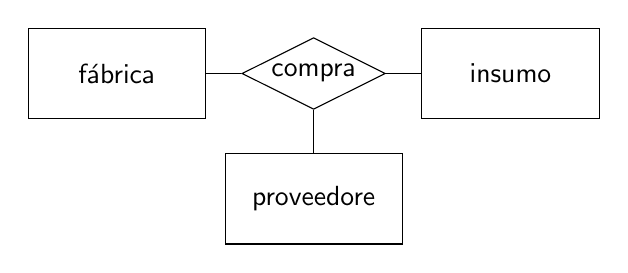
\begin{tikzpicture}[font=\sffamily]
	\node[draw,minimum width=2.25cm,minimum height=1.15cm] (ent1) at (0,0) {fábrica};
	\node[draw,minimum width=2.25cm,minimum height=1.15cm] (ent2) at (5,0) {insumo};
	\node[draw,minimum width=2.25cm,minimum height=1.15cm] (ent3) at (2.5,-1.59) {proveedore};
	\node[draw,shape aspect=2,diamond,inner sep=0.5mm] (rel) at (2.5,0) {compra};
	\draw (ent1)--(rel)--(ent2) (rel)--(ent3);
\end{tikzpicture}

\end{document}
